In this section we will give a detailed walk-through of an integration case study. We will show how to use the graph anonymization library in an existing Go code base. This existing code base is a containerized anonymization system leveraging the MongoDb document database. It was developed by \emph{Vilmos Sz. Martinek} as part of his MSc thesis while studying at \textit{Budapest University of Technology and Economics} in 2018~\cite{martinek}. A cornerstone of the integration is to make the \emph{minimum amount of changes} in the existing system, while introducing an alternative anonymization algorithm as an optionally selectable component.

\subsection{Overview of the target system}

The target anonymization system implements a standard three-tiered architecture. See Figure~\ref{fig:integration_arch}. We highlighted network boundaries with blue dashed lines on the figure.

\subsubsection{REST API}\label{subsubsec:rest_api}
Client applications can use the system through a provided REST API, which supports two operations: \emph{data set creation} and \emph{data upload}. The former makes it possible to push data into different MongoDb collections, the latter deals with actually receiving the data in the form of JSON documents.

\vspace{\baselineskip}
\begin{figure}[H]
    \centering


\tikzset{every picture/.style={line width=0.75pt}} %set default line width to 0.75pt

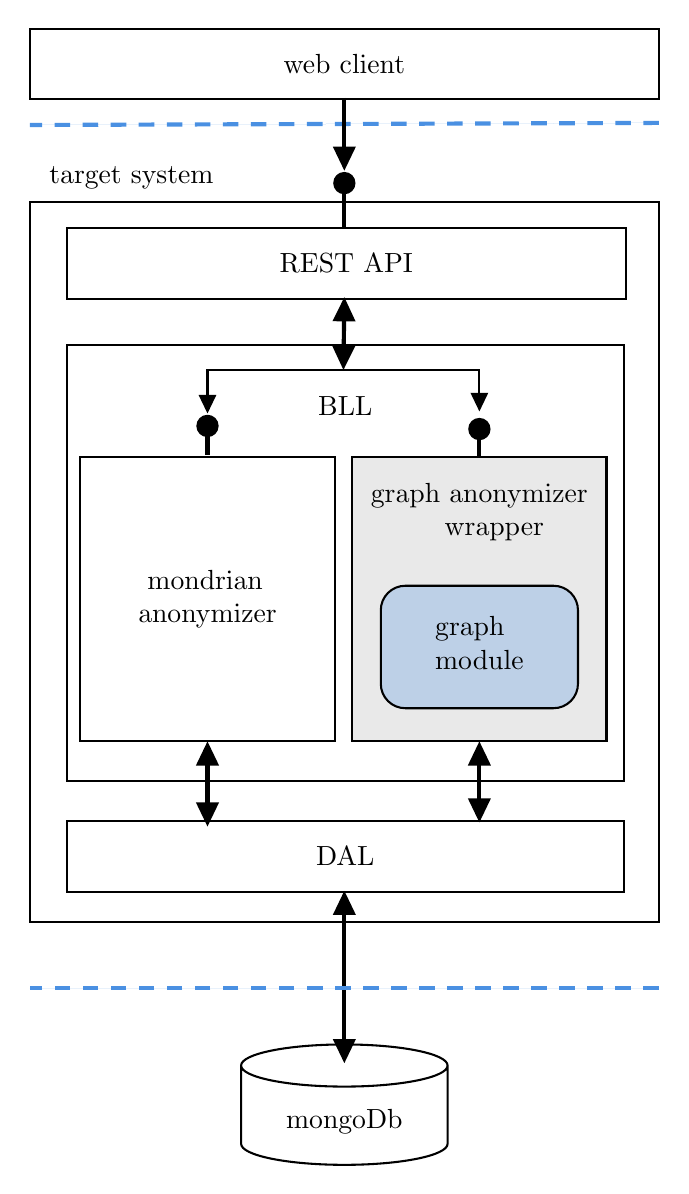
\begin{tikzpicture}[x=0.75pt,y=0.75pt,yscale=-1,xscale=1]
%uncomment if require: \path (0,571); %set diagram left start at 0, and has height of 571

%Shape: Rectangle [id:dp25314219983411235]
\draw  [fill={rgb, 255:red, 155; green, 155; blue, 155 }  ,fill opacity=0.22 ] (349.75,216) -- (472.25,216) -- (472.25,353) -- (349.75,353) -- cycle ;
%Rounded Rect [id:dp6104192131332256]
\draw  [fill={rgb, 255:red, 74; green, 144; blue, 226 }  ,fill opacity=0.28 ] (363.5,289.8) .. controls (363.5,283.28) and (368.78,278) .. (375.3,278) -- (446.7,278) .. controls (453.22,278) and (458.5,283.28) .. (458.5,289.8) -- (458.5,325.2) .. controls (458.5,331.72) and (453.22,337) .. (446.7,337) -- (375.3,337) .. controls (368.78,337) and (363.5,331.72) .. (363.5,325.2) -- cycle ;
%Shape: Rectangle [id:dp7542396041522255]
\draw   (194.38,9.62) -- (497.5,9.62) -- (497.5,43.63) -- (194.38,43.63) -- cycle ;

%Shape: Rectangle [id:dp8775304827751447]
\draw   (194.37,93) -- (497.5,93) -- (497.5,440) -- (194.37,440) -- cycle ;
%Shape: Rectangle [id:dp29329734503174665]
\draw   (212.25,105.63) -- (481.5,105.63) -- (481.5,139.63) -- (212.25,139.63) -- cycle ;

%Shape: Rectangle [id:dp3924156131636001]
\draw   (212.25,162) -- (480.5,162) -- (480.5,372) -- (212.25,372) -- cycle ;
%Shape: Rectangle [id:dp02053336225786917]
\draw   (212.25,391.41) -- (480.5,391.41) -- (480.5,425.41) -- (212.25,425.41) -- cycle ;

%Shape: Rectangle [id:dp8663149504803358]
\draw   (218.75,216) -- (341.25,216) -- (341.25,353) -- (218.75,353) -- cycle ;
%Flowchart: Magnetic Disk [id:dp36269861006508]
\draw   (395.69,509.15) -- (395.69,546.85) .. controls (395.69,552.46) and (373.41,557) .. (345.94,557) .. controls (318.46,557) and (296.19,552.46) .. (296.19,546.85) -- (296.19,509.15)(395.69,509.15) .. controls (395.69,514.76) and (373.41,519.3) .. (345.94,519.3) .. controls (318.46,519.3) and (296.19,514.76) .. (296.19,509.15) .. controls (296.19,503.54) and (318.46,499) .. (345.94,499) .. controls (373.41,499) and (395.69,503.54) .. (395.69,509.15) -- cycle ;

%Straight Lines [id:da08877933566463603]
\draw [color={rgb, 255:red, 74; green, 144; blue, 226 }  ,draw opacity=1 ][fill={rgb, 255:red, 74; green, 144; blue, 226 }  ,fill opacity=1 ][line width=1.5]  [dash pattern={on 5.63pt off 4.5pt}]  (497.5,55) -- (194.38,56) ;


%Straight Lines [id:da5932184702081]
\draw [line width=1.5]    (345.94,84) -- (345.94,105) ;

\draw [shift={(345.94,84)}, rotate = 90] [color={rgb, 255:red, 0; green, 0; blue, 0 }  ][fill={rgb, 255:red, 0; green, 0; blue, 0 }  ][line width=1.5]      (0, 0) circle [x radius= 4.36, y radius= 4.36]   ;
%Straight Lines [id:da8662427461600262]
\draw [line width=1.5]    (345.94,43) -- (345.94,75) ;
\draw [shift={(345.94,78)}, rotate = 270] [fill={rgb, 255:red, 0; green, 0; blue, 0 }  ][line width=1.5]  [draw opacity=0] (11.61,-5.58) -- (0,0) -- (11.61,5.58) -- cycle    ;

%Straight Lines [id:da5790521830826718]
\draw [line width=1.5]    (345.94,428) -- (345.94,505) ;
\draw [shift={(345.94,508)}, rotate = 270] [fill={rgb, 255:red, 0; green, 0; blue, 0 }  ][line width=1.5]  [draw opacity=0] (11.61,-5.58) -- (0,0) -- (11.61,5.58) -- cycle    ;
\draw [shift={(345.94,425)}, rotate = 90] [fill={rgb, 255:red, 0; green, 0; blue, 0 }  ][line width=1.5]  [draw opacity=0] (11.61,-5.58) -- (0,0) -- (11.61,5.58) -- cycle    ;
%Straight Lines [id:da9813732944058937]
\draw [line width=1.5]    (345.9,142) -- (345.54,171) ;
\draw [shift={(345.5,174)}, rotate = 270.72] [fill={rgb, 255:red, 0; green, 0; blue, 0 }  ][line width=1.5]  [draw opacity=0] (11.61,-5.58) -- (0,0) -- (11.61,5.58) -- cycle    ;
\draw [shift={(345.94,139)}, rotate = 90.72] [fill={rgb, 255:red, 0; green, 0; blue, 0 }  ][line width=1.5]  [draw opacity=0] (11.61,-5.58) -- (0,0) -- (11.61,5.58) -- cycle    ;
%Straight Lines [id:da5100456793816999]
\draw [line width=1.5]    (280,356) -- (280,391) ;
\draw [shift={(280,394)}, rotate = 270] [fill={rgb, 255:red, 0; green, 0; blue, 0 }  ][line width=1.5]  [draw opacity=0] (11.61,-5.58) -- (0,0) -- (11.61,5.58) -- cycle    ;
\draw [shift={(280,353)}, rotate = 90] [fill={rgb, 255:red, 0; green, 0; blue, 0 }  ][line width=1.5]  [draw opacity=0] (11.61,-5.58) -- (0,0) -- (11.61,5.58) -- cycle    ;
%Straight Lines [id:da9511987307073959]
\draw [color={rgb, 255:red, 74; green, 144; blue, 226 }  ,draw opacity=1 ][fill={rgb, 255:red, 74; green, 144; blue, 226 }  ,fill opacity=1 ][line width=1.5]  [dash pattern={on 5.63pt off 4.5pt}]  (497.5,472) -- (194.37,472) ;


%Straight Lines [id:da6634746570080241]
\draw [line width=1.5]    (280,201) -- (280,215) ;

\draw [shift={(280,201)}, rotate = 90] [color={rgb, 255:red, 0; green, 0; blue, 0 }  ][fill={rgb, 255:red, 0; green, 0; blue, 0 }  ][line width=1.5]      (0, 0) circle [x radius= 4.36, y radius= 4.36]   ;
%Straight Lines [id:da11396993553443457]
\draw [line width=1.5]    (411,202.5) -- (411,216.5) ;

\draw [shift={(411,202.5)}, rotate = 90] [color={rgb, 255:red, 0; green, 0; blue, 0 }  ][fill={rgb, 255:red, 0; green, 0; blue, 0 }  ][line width=1.5]      (0, 0) circle [x radius= 4.36, y radius= 4.36]   ;
%Straight Lines [id:da6497437274365285]
\draw [line width=1.5]    (411,356) -- (411,389) ;
\draw [shift={(411,392)}, rotate = 270] [fill={rgb, 255:red, 0; green, 0; blue, 0 }  ][line width=1.5]  [draw opacity=0] (11.61,-5.58) -- (0,0) -- (11.61,5.58) -- cycle    ;
\draw [shift={(411,353)}, rotate = 90] [fill={rgb, 255:red, 0; green, 0; blue, 0 }  ][line width=1.5]  [draw opacity=0] (11.61,-5.58) -- (0,0) -- (11.61,5.58) -- cycle    ;
%Straight Lines [id:da30407000837324416]
\draw    (280,193) -- (280,174) -- (411,174) -- (411,192) ;
\draw [shift={(411,194)}, rotate = 270] [fill={rgb, 255:red, 0; green, 0; blue, 0 }  ][line width=0.75]  [draw opacity=0] (8.93,-4.29) -- (0,0) -- (8.93,4.29) -- cycle    ;
\draw [shift={(280,195)}, rotate = 270] [fill={rgb, 255:red, 0; green, 0; blue, 0 }  ][line width=0.75]  [draw opacity=0] (8.93,-4.29) -- (0,0) -- (8.93,4.29) -- cycle    ;

% Text Node
\draw (411,305.5) node [scale=1] [align=left] { graph\\module};
% Text Node
\draw (243.38,81.25) node  [align=left] {target system};
% Text Node
\draw (346.88,122.63) node  [align=left] {REST API};
% Text Node
\draw (346.37,408.41) node  [align=left] {DAL};
% Text Node
\draw (346.38,191.63) node  [align=left] {BLL};
% Text Node
\draw (280,284.5) node  [align=left] { \ mondrian\\anonymizer};
% Text Node
\draw (411,242.63) node  [align=left] {graph anonymizer\\ \ \ \ \ \ \ \ \ wrapper};
% Text Node
\draw (345.94,536) node  [align=left] {mongoDb};
% Text Node
\draw (345.94,26.63) node  [align=left] {web client};


\end{tikzpicture}
    \caption{Integration with the target system}\label{fig:integration_arch}
\end{figure}

\subsubsection{BLL}
The business logic layer contains the anonymization related code. This is where we need to implement the integration with the graph based anonymizer. Initially the system supported a single anonymization algorithm, called \emph{Mondrian}. Mondrian is a top-down greedy anonymization algorithm, which uses a \emph{kd-tree} to partition the raw data into partitions for generalization. In this document we will not discuss the Mondrian algorithm in further details --- we can simply think about it as another anonymization algorithm with different characteristics than the graph based anonymizer. In certain circumstances it might be beneficial to use one versus the other, so it would be useful to be able to switch between the two types of algorithms for different data sets.

The BLL layer already contained an interface which encapsulates the public API of an anonymizer, hence the need for a \emph{wrapper} around the graph anonymizer. The wrapper provides a thin layer around the API introduced in Section~\ref{sec:example_run} and makes it compatible with the rest of the system.

\subsubsection{DAL}
The data access layer uses the \emph{mgo} third party library to interface with MongoDb. Since this layer is not the focus point for our integration case study, we will not detail its internals in this document.

\subsection{Adapting the input data format}\label{subsec:json_input_format}
As mentioned in~\ref{subsubsec:rest_api}, both the configuration and upload of the data is done through the REST API, so our first step will be to extend the input declaration, and make it able to switch between algorithms and configure parameters for both types of algorithms.

\paragraph{Original input format:} an example of the unmodified input format can be seen on Listing~\ref{lst:original_format}. The structure contains a \textit{settings} and \textit{fields} object. The former describes the anonymization parameters, the latter the field definitions (or \emph{schema}). Each field can have:
\begin{itemize}
    \setstretch{1.0}
    \item \textbf{name:} the name of the column
    \item \textbf{mode:} how the column should be treated. Can be \textit{id} or \textit{qid}
    \item \textbf{type:} data type for anonymization. Can be \textit{numeric}, \textit{prefix}
\end{itemize}

\vspace{\baselineskip}
\begin{lstlisting}[caption=Original input format,label=lst:original_format,float,floatplacement=H]
{
  "settings": {
    "k": 3,
    "algorithm": "mondrian",
    "mode": "single"
  },
  "fields": [
    {
      "name": "name",
      "mode": "qid",
      "type": "prefix"
    },
    // etc...
  ]
}
\end{lstlisting}


\paragraph{Modified input format:} fortunately the \textit{settings} object already supports defining the algorithm name (even though initially only the Mondrian value was supported), so this field can be reused. We can also reuse most of the field settings as well, however we need to introduce a couple of extra data types and also make it possible to configure the generalizers when selecting the graph anonymizer.

\vspace{\baselineskip}
\begin{lstlisting}[caption=Modified input format,label=lst:modified_format,float,floatplacement=H]
{
    "settings": {
        "k": 3,
        "algorithm": "graph",
        "mode": "single"
    },
    "fields": [
        {
            "name": "name",
            "mode": "drop"
        },
        {
            "name": "age",
            "mode": "qid",
            "type": "numeric",
            "opts": {
                "type": "int",
                "min": 0,
                "max": 150
            }
        },
        {
            "name": "salary",
            "mode": "qid",
            "type": "numeric",
            "opts": {
                "type": "float",
                "min": 0,
                "max": 200000
            }
        },
        {
            "name": "motto",
            "mode": "qid",
            "type": "prefix",
            "opts": {
                "max": 150
            }
        }
    ]
}
\end{lstlisting}



The modified input format is shown on Listing~\ref{lst:modified_format}. We now allow the \textit{``graph''} value for the \textit{algorithm} field. We also introduced the \textit{``keep''} and \textit{``drop''} values for the \textit{mode} field to be able to have a finer control over what columns to anonymize, leave alone, or suppress completely.

The field configuration objects now allow an \textit{``opts''} object. This will only be processed by the graph wrapper, the Mondrian module will ignore it entirely. This object contains graph anonymizer related parameters for certain field types (\textit{min}, \textit{max} values for range generalizers, and a \textit{max}-words setting for prefix generalizers).

\subsection{Implementing the wrapper}

The framework provides the \texttt{anonymizerAlgorithm} interface as an abstraction for the top level API of anonymization. Mondrian is an implementation of this interface, and we will need to implement the wrapper to be an implementation as well. Figure~\ref{lst:anon_interface} shows the interface.

\vspace{\baselineskip}
\begin{lstlisting}[caption=The \texttt{anonymizerAlgorithm interfcae},label=lst:anon_interface,float,floatplacement=H]
type anonymizerAlgorithm interface {
	initialize(*anonmodel.Dataset, string, []anonmodel.FieldAnonymizationInfo)
	anonymize() error
}
\end{lstlisting}

The \texttt{initialize} method is called by the framework after instantiating the anonymizer, but before calling the \texttt{anonymize} method. It gets the parsed settings for the fields and data set from the input JSON detailed in~\ref{subsec:json_input_format}. We can use this method to initialize the schema, since the modified JSON input now contains all the required information to declare the columns with the appropriate generalizer for each field. Note, that the actual data to anonymize is not passed to the wrapper by the framework (see~\ref{subsec:anonymizing_the_data}).

\subsection{Anonymizing the data}\label{subsec:anonymizing_the_data}

Recall from~\ref{subsubsec:rest_api}, that the client facing interface provided a separate web method for \emph{uploading data}. It is the responsibility of the implementor of \texttt{anonymizerAlgorithm} to get hold of the data for the data set specified in the parameters. In essence, the graph wrapper will need to have a reference to the DAL, and when the \texttt{anonymize} method is called by the framework, it must first query the data waiting to be anonymized. When the anonymization is finished, it should insert the anonymized data and mark it \emph{done}.

\subsection{Tests}

Finally, after the wrapper has been implemented, we needed to verify that the modified system is working correctly. The following types of testing have been performed:
\begin{itemize}
    \setstretch{1.0}
    \item \textbf{unit tests:} in these tests we need to mock the data access layer, and verify that input parsing, schema declaration and anonymization is working correctly.
    \item \textbf{regression:} normally we run the framework-provided unit test suite to verify, that we did not break any existing functionality. Unfortunately there were no unit tests in the original code base. This leaves us with the only option to first \emph{before touching anything} cover the most important parts of the original code base (for the original functionality) with tests, until a sufficient coverage rate is reached. \emph{Then} proceed with implementing our changes, where we can verify by running the test suite at any time that our added functionality is not breaking existing features. Before actually modifying the existing code base, I have taken a great care to cover as much of the original functionality as possible (see Figure~\ref{fig:tests_added}).
    \item \textbf{integration tests:} we verify, that integration between the BLL \& REST API, and BLL \& MongoDb isn't broken. We can do this by bringing up the system in the provided \emph{docker} container and calling the REST API with an HTTP client, or checking the data queried/inserted from/to the database respectively.
\end{itemize}

\vspace{\baselineskip}
In Go testing is built into the language and the core tooling. There is no need to depend on third party libraries, one can simply use the \texttt{testing} package. Tests can be invoked with the \texttt{go test} command which automates execution of any function which matches the required naming convention\cite{go-testing} of \texttt{func TestXxx (*testing.T)}. (See Listing~\ref{lst:go_test} for a basic example).

\begin{lstlisting}[caption=A basic Go test,label=lst:go_test,float,floatplacement=H]
package demo

import "testing"

func TestFactorial(t *testing.T) {
    fact := Factorial(5)
    if fact != 120 {
        t.Errorf("got: %d, want: %d.", fact, 120)
    }
}
\end{lstlisting}

A test suite can be crated by putting the test functions into a file whose name ends with \texttt{\_test.go}. This file needs to be in the same package as the one being tested. All tests will be excluded from regular package builds\cite{go-testing}, meaning that production artifacts will not be polluted with test files.

Actual test functions will rely on the \texttt{*testing.T} argument passed into the test function to interact with the testing framework. The testing toolkit follows the general philosophy of Go, being minimal, simple to use yet performant and robust.

\subsection{Verifying expectations}

When compared to testing libraries in other languages, the most obvious difference is the \emph{absence of assertions}. Code that checks expectations should be written explicitly, and the test should be terminated with a respective function call to \texttt{t.Error} or \texttt{t.Fail} when expectations aren't met.

But why isn't \texttt{assert} part of Go's testing package? One of the most important reasons is that the creators of the language wanted to avoid a common problem with other testing frameworks, namely that tests feel like they are written in a different language\cite{go-book}. They often have their own special syntax (like \textit{Mocha, RSpec}) which reads very differently from ``normal'' code.

\subsection{Special test types}

\subsubsection{Sub-test}
The testing package contains a \texttt{Run} method on the \texttt{testing.T} and \texttt{testing.B} types, that allows the creation of sub-tests and sub-benchmarks respectively. Sub-tests result in a more readable test code and provide a way to handle common setup for test cases.

\subsubsection{Table tests}
Table driven tests run the same logical test code for multiple similar test cases. In Go, table tests are implemented by declaring an array of test cases, then looping over them and running each iteration as a sub-test. This is called a table-driven test. (See Listing~\ref{lst:go_table_test}.)

\begin{lstlisting}[caption=Table-driven test,label=lst:go_table_test,float,floatplacement=H]
func TestFactorial(t *testing.T) {
    tests := []struct { n, want int }{
        {0, 1},
        {1, 1},
        {2, 2},
        {3, 6},
    }
    for _, test := range tests {
        t.Run("factorial test", func(t *testing.T) {
            // test logic
        })
    }
}
\end{lstlisting}

\subsubsection{Benchmarks}\label{subsec:benchmarks}
Benchmarks are special tests, with the goal of measuring the performance of a given function or code block. They are placed into \texttt{\_test.go} files, just like the normal tests, but their names start with the \texttt{Benchmark} word, and they get the \texttt{*testing.B} type as parameter. A typical benchmark runs the function \texttt{N} times, which value is provided by the benchmark runner. (It will increase the value until the spread is within a given margin of error.) The runner will also take care of calculating and printing the average execution time (ns/op). A skeleton of a typical benchmark is shown in Listing~\ref{lst:go_bench}. Note, that benchmarks can be combined well with table tests to perform a detailed analysis of a function for different kinds of arguments. We will use this feature heavily in Section~\ref{sec:benchmarks} when measuring the performance of the anonymization algorithm.

\begin{lstlisting}[caption=Go Benchmark,label=lst:go_bench,float,floatplacement=H]
func BenchmarkFactorial(b *testing.B) {
    for i:=0; i < b.N; i++ {
        // run the function
    }
}
\end{lstlisting}

\subsection{Coverage}
The Go testing framework has built-in support for statement coverage. It can be used in conjunction with \texttt{go test} by passing on the \texttt{-cover} flag. We generally aim to use test coverage as a metric to highlight edge-cases and missed branches during testing. Higher statement coverage is usually better, but it should be noted, that it is not an end-to-all metric. There can be missed test cases, or errors in the code even while having a 100\% statement coverage.